% ==============================================================================
%
%                          R E Q U I R E M E N T S
%
% ==============================================================================

\chapter{Graphical Front End} % <<< ------------------------------------------ %
\label{ch:graphical_front_end}

To view measured data a oscilloscope application (scope in further text) with a graphical user interface (GUI in further text) and mathematical capabilities like calculating the spectral density or the SNR of the signal was created. It can receive the recorded samples over the network and display them on a canvas. Furthermore it manages triggers and does a lot of math to get more specific metrics of a signal.
In this section the requirements for this piece of software, the design choices and the implementation details as well as the results are discussed.

\section{Requirements}
\label{sec:gui:requirements}

The requirements for the scope were given by the scoping application ``Spektrum Analyzer'' TODO: cite?? written in Java by Prof. Gut and his students.
The task description required the new scope to have the same features as the old one plus as many more as possible.

The requirements were as follows

\begin{itemize}
    \item Receive data in configurable size over the network.
    \item Display received data in time as well as fequency space.
    \item Calculate the RMS power density in the signal.
    \item Calculate the THD ratio of the signal.
\end{itemize}

% ==============================================================================
%
%                         D E S I G N   C H O I C E S
%
% ==============================================================================

\section{Design Choices}
\label{sec:gui:design_choices}

There is a wealth of programming languages to choose from but only a few suit a task best. And there are as many libraries helping with graphics and networking as well for most of those languages.
In the following sections explain why JavaScript and web technologies are used to implement a GUI and mathematical functions in this project.

A select few popular programming languages have been evaluated. They have been given weights for certain attributes of the respective language to determine the best fitting one. The results are visible in the comparison matrix~\ref{fig:gui:language_choices}.

All the attributes with their impact and meaning for this project are explained in the following.

\subsection*{Open Standard} Since this is a university based project meant for educational purposes too, it is very important to make all source code available under public license. Thus it is important to have a company and paid model independant solution. Many languages are managed by a council or similar and open to public commits and thus deemed an open standard. Some are managed by a company and not classiefied as a open standard.

\subsection*{Networking} To ensure a fast and lossless data transfer, it was very important to have the choice between good networking protocols as well as convenient libraries to ease the use of those standards.
Networking is not a trivial thing and standards can be quite engineering- and feature-heavy. Thus it is important to have ready-to-use libraries that abstract the network. For more information on evaluated networking solutions, read Section~\ref{subsec:gui:networking}.

\subsection*{Graphics} An oscilloscope is quite requiring when it comes to graphics, since a image-stream that is fluent for the human eye has to be provided in a high resolution. This fact made it indispensable to use a library that interfaces OpenGL. Since a interface is not easy to design from scratch only using rectangles and circles, a GUI toolkit that makes the design process of the GUI easy is indispensable.

\subsection*{Widespread} It is important for the project to use a widespread solution since that way it is easy to obtain information and ask more savy users about certain pitfalls.

\subsection*{User-Friendly} Some solutions are more user-friendly when it comes to toolkits and usage. Since both team members come form a Linux background, it was strongly preferred to use a language that does not quasi-require a huge IDE or requires a lot of uneasy maintenance.

\subsection*{Easy To Use(r)} Since not all users want to fight with installers and package managers, the deployment options as well as general stability of the environment for the binaries were a strong point in the descision process.

\subsection*{Familiarity With The Language} The best toolkits do not matter if none of the involved programmers have ever used it and will struggle with even the basics for a major part of the project duration. Thus it was unavoidable to have some personal preferences for some languages.

\begin{table}
\begin{centering}
\setlength{\extrarowheight}{2pt}
\begin{tabular}{*{7}{c|}}
    \multicolumn{2}{c}{}        & \multicolumn{2}{c}{}\\\cline{3-7}
    \multicolumn{1}{c}{}    &   & \parbox[t]{2mm}{\rotatebox[origin=c]{90}{Rust}}%
                                & \parbox[t]{2mm}{\rotatebox[origin=c]{90}{C++}}%
                                & \parbox[t]{2mm}{\rotatebox[origin=c]{90}{Java}}%
                                & \parbox[t]{2mm}{\rotatebox[origin=c]{90}{Python}}%
                                & \parbox[t]{2mm}{\rotatebox[origin=c]{90}{JavaScript}} \\\cline{2-7}
                & Open Standard & 6 & 6 & 1 & 6 & 6\\\cline{2-7}
                   & Networking & 6 & 6 & 6 & 6 & 4\\\cline{2-7}
                     & Graphics & 2 & 5 & 5 & 5 & 6\\\cline{2-7}
                   & Widespread & 3 & 6 & 6 & 5 & 6\\\cline{2-7}
                & User-Friendly & 5 & 5 & 5 & 5 & 6\\\cline{2-7}
               & Easy To Use(r) & 3 & 4 & 5 & 6 & 6\\\cline{2-7}
& Familiarity With The Language & 3 & 3 & 4 & 6 & 6\\\cline{2-7}
                       & Total &28 &35 &32 &39 & 40\\\cline{2-7}
\end{tabular}
\caption{Weights of certain aspects of possible programming languages.}
\label{fig:gui:language_choices}
\end{centering}
\end{table}

After weighting in all the different aspects JavaScript was chosen as the language to implement the oscilloscope. JavaScript is a scripting language that can be interpreted by the browser.
It is known for it's high versatility and widespread use in the web community.
A few years ago, JavaScript would not have been a viable choice for graphics and networking at all. But with the recent addition, and more important, great increase in stability and performance of WebGL and WebSockets JavaScript has become a very potent solution available to everyone.
With JavaScript deploying the application to the enduser is as simple as making it accessible via a website that runs on the STEMlab board. Thus it is very convenient for the user to work with the board, considering the assumption that every user has a webbrowser that is able to run the application.
A downside of JavaScript is the huge runtime the browser needs to execute the application and thus resulting in a lot of memory ressources used. Since those are easily available nowadays, this issue was considered non-relevant.
Another downside of JavaScript is that it leaves very little room when it comes to networking choices. For streaming data there is only WebSockets that performs well. Since WebSockets is a very capable and convenient solution, this issue did not change much in the descision process.

% ==============================================================================
%
%                          N E T W O R K I N G
%
% ==============================================================================

\subsection{Networking}
\label{subsec:gui:networking}

To ensure a fluent stream of data, very little overhead for the transmitted data is key.

Normally for streamed data \textit{where packets can be lost}, \textbf{UDP} is the best choice since it has no overhead for guaranteeing completeness and in-order for all packets sent.
UDP sends packets but does not guarantee that none are lost.

For guaranteed transmission and sequentiality of the data, one is advised to use \textbf{TCP}. This comes at the cost of some more overhead. This overhead is most of the time completely negligible as a custom solution that performs better than TCP is very hard to write. What TCP does more that is important for this project is congestion control. It ensures that no more packets are sent if old ones are missing. It prevents the network from collapsing because an UDP sender sends all packets it can and thus using the entire bandwidth even if the receiver cannot even process the data at this point.
This means that TCP also helps when the bandwith is small by waiting for the current package and not already sending further packages and thus providing sort of automatic bandwith adaption.
There is the possibility of using raw TCP sockets or one of TCP's subprotocols. Raw sockets require the user to implement their own protocol entirely to handle data transmission on an application layer whilst using subprotocols already provide a standard way to do so.
Two of those subprotocols are HTTP and WebSockets. HTTP comes with great overhead and is meant for single transactions only. It does not fit the project's needs.
WebSockets on the contrary are meant for data streaming and fit the project's needs precisely.
Since JavaScript cannot use raw TCP sockets and needs WebSockets to espablish a raw-ish TCP socket, this is the chosen solution, as it has not downsides relevant for this project.
The functionality of WebSockets is explained a little bit more in the subsection~\ref{subsec:gui:websockets}.

% ==============================================================================
%
%                              P R O D U C T
%
% ==============================================================================

\subsection{Product}
\label{sec:gui:product}

\begin{figure}
    \centering
    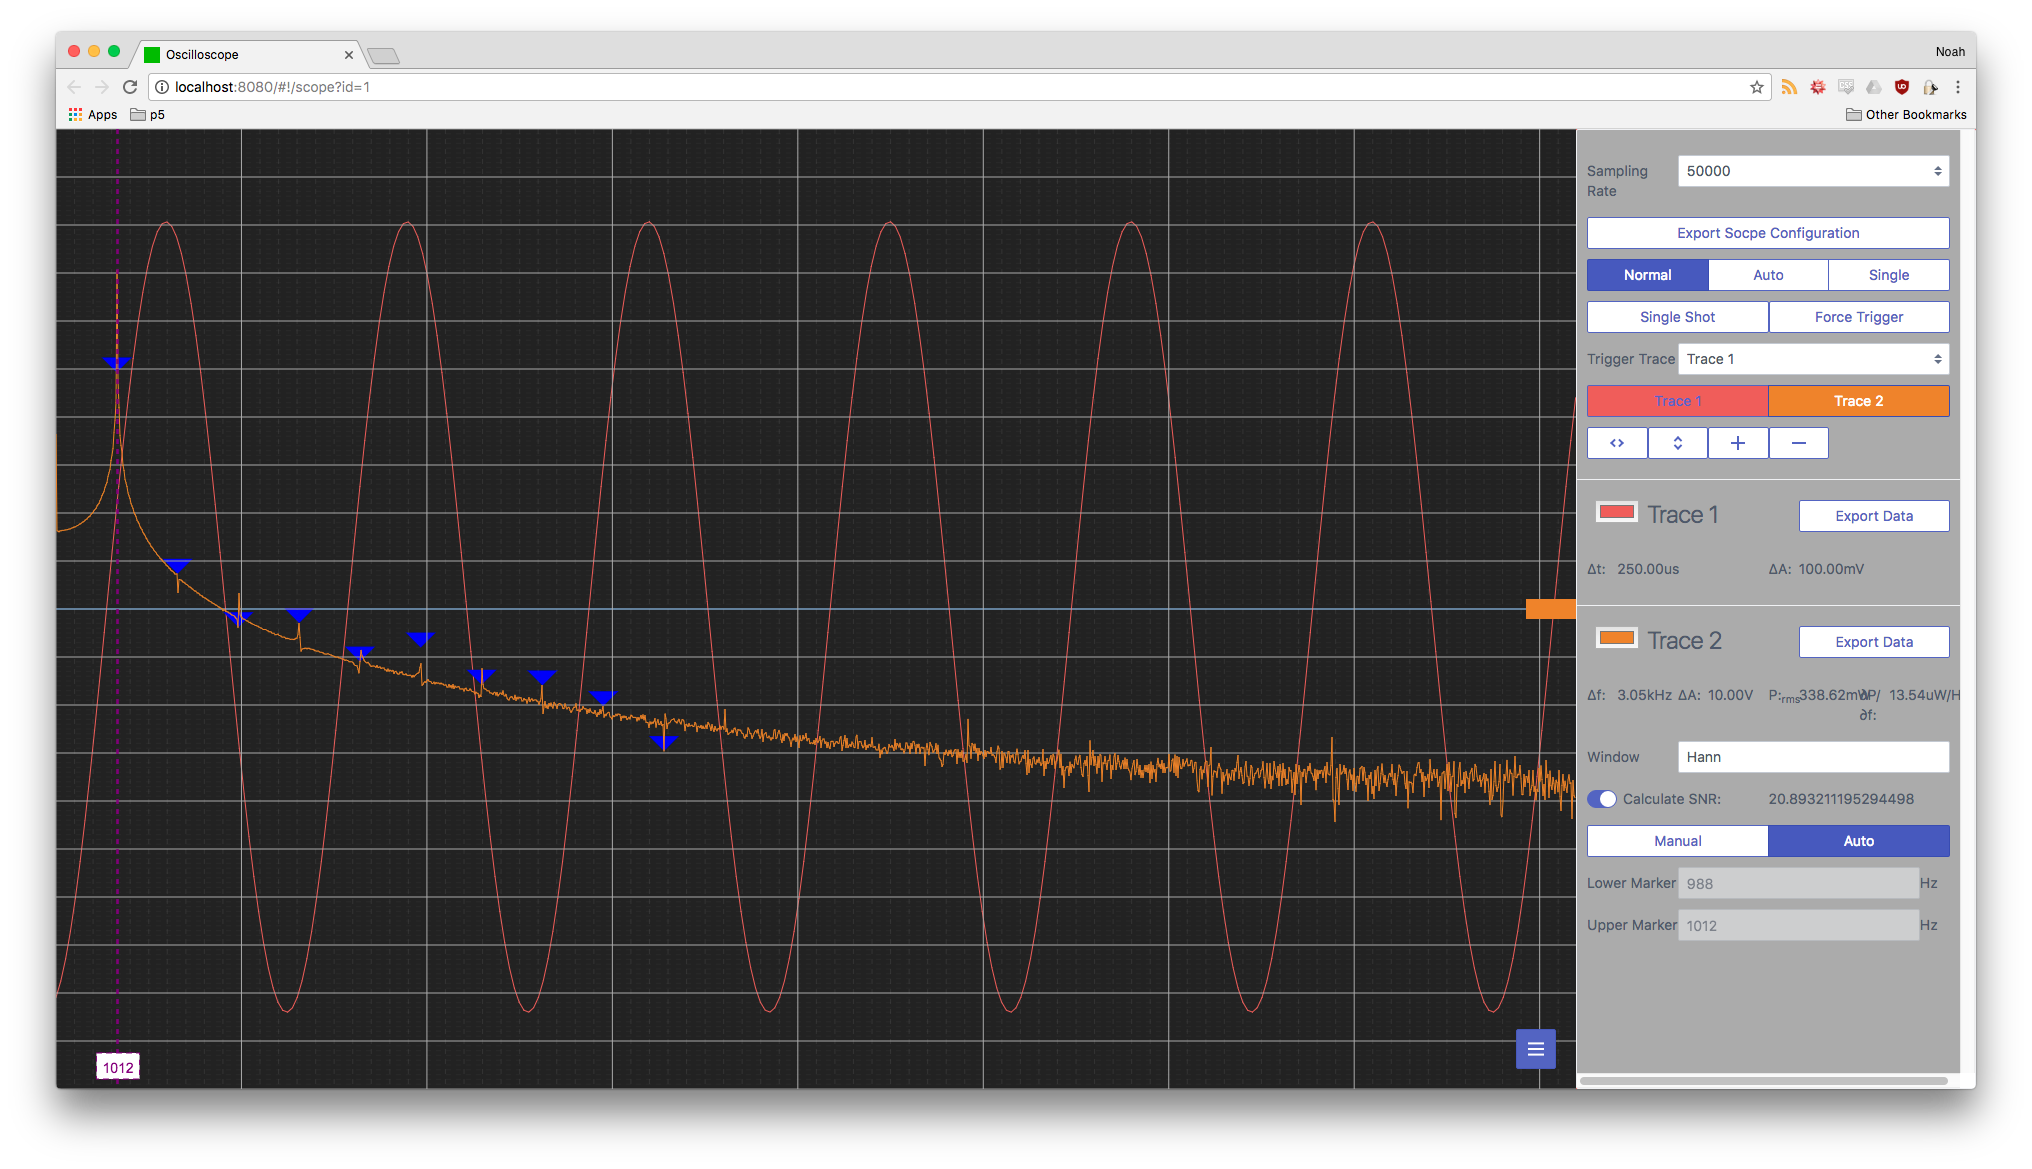
\includegraphics[width=1\textwidth]{images/gui/scope}
    \caption[The scope application]{%
        The scope application in it's current state, displaying time and FFT data.%
    }
    \label{fig:gui:structure}
\end{figure}

The oscilloscope application is a web application that can be directly loaded from the server running on the STEMlab.
It is capable of the following things as of date:

\begin{itemize}
    \item Receive data over the network for two channels (this is only limitted by the physical channels of the STEMlab).
    \item Manage triggering including setting a trigger type, level and a number of samples that have to be recorded before and after the trigger was issued.
    \item Calculate and display the power density spectrum.
    \item Calculate the SNR both automatically detecting the signal and manually being told where the signal is.
    \item Calculate the THD for a given base harmonic. TODO: !
    \item Export data to an array-string.
    \item Export and load the scope configuration to and from JSON strings.
\end{itemize}

How the application is structured and certain features are implemented is explained in the following sections.

% ==============================================================================
%
%                  A P P L I C A T I O N   S T R U C T U R E
%
% ==============================================================================

\subsection{Application Structure}
\label{subsec:gui:application_structure}

The entire application consists of a single state tree. This makes it very easy to import and export settings on one hand and on the other it concentrates all the states in one place which gives a way better overview than in the case all the states are scattered in various objects in the application.
Listing~\ref{lst:gui:app_structure} shows an extract of the tree structure.

As every JavaScript application this application runs asynchronous too. The entire eventloop structure can be seen in Figure~\ref{fig:gui:eventloop}.

\begin{figure}
    \centering
    \begin{tikzpicture}[%
        align=center,
        text=q1,
        draw=sq5,
    ]
    \small
    \sffamily

    \begin{scope}[
        every node/.style = draw,
        terminal/.append style={
            rounded rectangle,
            fill=sq5,
            text=q1,
            inner sep=2mm,
        }, % data packages
        sign/.style={
            inner sep=2mm,
            rounded corners=1mm,
            fill=sq5,
            text=q1,
        },         % custom signal style
        circ/.style={
            inner sep=2mm,
            rounded corners=1mm,
            double,
            fill=sq5,
            draw=q1,
            text=q1,
        }, % circuitry
        proc/.style={
            inner sep=2mm,
            rounded corners=1mm,
            fill=sq5,
            text=q1,
        },       % process/activity
        dec/.style={
            inner sep=2mm,
            rounded corners=1mm,
            fill=sq5,
            text=q1,
        },       % decision/activity
        stor/.style={
            fill=cyan!30
        },         % storage
        dbtable/.style={
            text=sq5,
            draw=q1,
            rounded corners=1mm,
            inner sep=2mm,
        } % database tables
    ]
        \node (newUART) [
            dec,
            align=center,
            diamond,
            minimum width=33mm,
            minimum height=33mm,
        ] at (0,0) {neuer\\UART\\Request?};
        \node (init) [
            proc,
            above=of newUART,
            align=center,
        ] {Hardware\\initialisieren};
        \node (forMe) [
            dec,
            align=center,
            diamond,
            right=of newUART,
            minimum width=33mm,
            minimum height=33mm,
        ] {F\"ur mich?};
        \node (package) [
            proc,
            right=of forMe,
            align=center,
        ] {Datenpaket mit\\Moving Average\\ und Addresse\\erstellen};
        \node (crc) [
            proc,
            below=of package,
            align=center,
        ] {CRC brechnen\\und zu Daten\\hinzuf\"ugen};
        \node (send) [
            proc,
            left=of crc,
            align=center,
        ] {Datenpaket\\senden};
        \node (getADC) [
            proc,
            below=of send,
            align=center,
        ] {ADC-Messung\\ausf\"uhren};
        \node (movAvg) [
            proc,
            below right=of getADC,
            align=center,
        ] {Moving\\Average\\berechnen};
        \node (LED) [
            proc,
            below left=of movAvg,
            align=center,
        ] {LED\\blinken\\lassen};
        \node (systick) [
            proc,
            above left=of LED,
            align=center,
        ] {auf n\"achsten\\\texttt{systick} warten};
    \end{scope}

    \begin{scope}[
            rounded corners,
            every path/.append style={draw=q1,},
            >=latex',
    ]
        \draw[-latex] (init) -- (newUART);
        \draw[-latex] (newUART) -- node[midway,anchor=south] {ja} (forMe);
        \draw[-latex] (forMe) -- node[midway,anchor=south] {ja} (package);
        \draw[-latex] (package) -- (crc);
        \draw[-latex] (crc) -- (send);
        \draw[-latex] (forMe) edge[bend left] node[midway,anchor=north] {nein} (newUART);
        \draw[-latex] (send) edge[bend left] (newUART);
        \draw (newUART) edge[loop below]  node {nein} (newUART);

        \draw[-latex] (getADC) edge[bend left] (movAvg);
        \draw[-latex] (movAvg) edge[bend left] (LED);
        \draw[-latex] (LED) edge[bend left] (systick);
        \draw[-latex] (systick) edge[bend left] (getADC);

    \end{scope}

\end{tikzpicture}
    \caption[Scope event structure]{%
        The scope event structure.%
    }
    \label{fig:gui:eventstructure}
\end{figure}

\begin{tcolorbox}[
        title={
            \refstepcounter{listing}
            Listing \thelisting: The state tree of the scope application
            \label{lst:gui:app_structure}
            \addcontentsline{lol}{listing}{\protect\numberline{\thelisting}}
        }
    ]
    \inputminted[
        linenos,
        numbersep=4pt,
        style=solarizedlight,
    ]{javascript}{./code/statetree.js}
\end{tcolorbox}

All of the values that can be controlled through the GUI - and many more - are also controllable directly through the state tree.
On application start the entire statetree is loaded and references to extracts of it are handed to the controller objects.

The structure of the application is hierarchical and the most important relations are depicted in Figure~\ref{fig:gui:structure}.

\begin{figure}
    \centering
    \tikzsetnextfilename{gui-structure}
\begin{tikzpicture}[%
    %show background grid,
    font=\small,
]
    \begin{class}[text width=4.5cm]{Oscilloscope}{0,0}
        \operation{draw(void)}
    \end{class}
    \begin{class}[text width=4.5cm]{Source}{0,-3}
        \operation{forceTrigger(void)}
        \operation{samplingRate(s: u32)}
        \operation{frameConfiguration(frameSize: u32, pre: u32, suf: u32)}
        \operation{triggerOn(trigger: Trigger)}
        \operation{single(channel: u32)}
        \operation{normal(channel: u32)}
        \operation{auto(channel: u32, timeout: u32)}
    \end{class}
    \begin{class}[text width=4.5cm]{WebSocketSource}{6,-4.15}
        \inherit{Source}
        \operation{sendJSON(string: String)}
        \operation{onOpen(void)}
        \operation{onMessage(e: Event)}
    \end{class}
    \begin{class}[text width=4.5cm]{Trace}{0,-9}
        \operation{draw(canvas: Canvas)}
        \operation{calc(void)}
    \end{class}
    \begin{class}[text width=4.5cm]{TimeTrace}{6,-8.7}
        %\inherit{Trace}
    \end{class}
    \begin{class}[text width=4.5cm]{FFTrace}{6,-10.3}
        %\inherit{Trace}
    \end{class}
    \begin{class}[text width=4.5cm]{GeneralPrefPane}{6,-0.3}
    \end{class}
    \begin{class}[text width=4.5cm]{TimeTracePrefPane}{6,-7.2}
    \end{class}
    \begin{class}[text width=4.5cm]{FFTracePrefPane}{6,-11.8}
    \end{class}
    %\composition{Oscilloscope}{source}{1}{Source}
    \composition{Oscilloscope}{}{}{Source}
    \composition{Source}{}{}{Trace}
    \composition{Oscilloscope}{}{1}{GeneralPrefPane}
    \composition{TimeTrace}{}{}{TimeTracePrefPane}
    \composition{FFTrace}{}{}{FFTracePrefPane}

    \node[text=black,anchor=west] at ($(Oscilloscope.south) - (0,2ex)$) {source};
    \node[text=black,anchor=east] at ($(Source.north) + (0,1.5ex)$) {1};
    \node[text=black,anchor=west] at ($(Source.south) - (0,2ex)$) {traces};
    \node[text=black,anchor=east] at ($(Trace.north) + (0,1.5ex)$) {1..*};
    \node[text=black,anchor=east] at ($(FFTracePrefPane.north) + (0,1.5ex)$) {1};
    \node[text=black,anchor=east] at ($(TimeTracePrefPane.south) - (0,2ex)$) {1};

    \draw [umlcd style inherit line] ($(Trace.east) + (0,1.5mm)$) -| (TimeTrace.south);
    \draw [umlcd style inherit line] ($(Trace.east) - (0,1.5mm)$) -| (FFTrace.north);
\end{tikzpicture}

    \caption[The scope structure]{%
        The structure of the scope application with all it's important relations.%
    }
    \label{fig:gui:structure}
\end{figure}

In the following some of the more important prototypes and functions are elaborated on.

% ==============================================================================
%
%                                  N O D E S
%
% ==============================================================================

\subsubsection*{Oscilloscope}

The Oscilloscope prototype is the top level controller which contains exactly one source. It is responsible for handling all mouse event and react accordingly, such as moving the trigger level or zooming and paning.
The Oscilloscope draw call is responsible for drawing general info on the canvas that is not part of a specific trace.
It is also the caller for the Trace draw call. The oscilloscope manages general information and is responsible for rescaling the canvas and initiating the draw call chain.

\subsubsection*{Source}

The Source controller manages all calls from and to the server. It contains a lot of helper calls to set a trigger or issue a new frame that are called by the Oscilloscope controller or GUI elements.
It also contains the important callbacks to send and receive data from the server which are explained in Section~\ref{subsec:gui:websockets}.
The source stores all received frames on itself which then, later in the call chain, will be copied and worked on by the trace controller.
Each frame received will always be overridden by the next one, ensuring no memory leaks and current data.
Once the Source controller received new data it starts the \textit{calc()} call for each trace to have them update the trace math with the new data.
In the next section the concept of WebSockes is explained very briefly. 

% ==============================================================================
%
%                             W E B S O C K E T S
%
% ==============================================================================

\subsubsection{WebSockets}
\label{subsec:gui:websockets}

WebSockets' final RFC 6455\cite{rfc:6455} was released in December 2011 and is thus still quite young. It is meant to compensate the lack of raw UDP and TCP sockets in JavaScript which is due to security threats that are not further elaborated here.
WebSockets is located in the Application Layer of the OSI model\footnote{For those not familiar with the OSI model Wikipedia~\ref{wiki:osi} provides a good overview.}.
Instead of directly opening a raw WebSocket, the handshake is done via HTTP(S). This brings the benefit of communicating through the same ports as the browser (80 or 443) which enables the protocol to go through most firewalls. Furthermore it greatly simplifies the handshake for the user (here being the programmer).
The client sends an upgrade request to the server which then opens a WebSocket connection.
This allows for a very conventient way to use TCP Sockets without any entirely new standards.
The section ``1.5 Design Philosophy'' in RFC 6455\cite{rfc:6455} explains it very well:

``Basically it is intended to be as close to just exposing raw TCP to script as possible given the constraints of the Web.

The only exception is that WebSockets adds framing to make it packet rather than stream based and to differentiate between binary and text data.
This differentiation is very useful for this project. Instructions to the server are issued via the text channel whilst data is sent back through the binary channel, allowing for very convenient interfacing with close to no effort.''

So in short: WebSockets are close-to-raw TCP sockets whose handle is shared through HTTP(S).
JavaScript provides a interface that makes it really easy to shove data back and forth.
As nearly anything in JavaScript this is done using callbacks. There is callbacks that handle connections, messages and errors. The code snippet in \ref{lst:gui:jsws} gives some insight how WebSockets in JavaScript are used. All the details can be read in the Mozilla documentation \cite{moz:ws}.

\begin{tcolorbox}[
        title={
            \refstepcounter{listing}
            Listing \thelisting: JavaScript ``Using WebSockets''
            \label{lst:gui:jsws}
            \addcontentsline{lol}{listing}{\protect\numberline{\thelisting}}
        }
    ]
    \inputminted[
        linenos,
        numbersep=4pt,
        style=solarizedlight,
    ]{javascript}{./code/websockets.js}
\end{tcolorbox}

\subsubsection*{Trace}

The Trace prototype is in charge of displaying the recorded and calculated data in the scope application.
The trace controller can be managing an FFT or a normal Time trace. This could be extensible to general math traces e.g. subtracting two differential pair traces for noise cancelling in the future.
Each derived trace prototype calculates some metrics and a grid to quantize the signal.

Whilst the Timetrace prototype just returns untouched data, the FFTrace prototype calculates metrics. Namely those are:

\begin{itemize}
    \item The spectral power density
    \item The SNR
    \item The THD TODO: !
\end{itemize}

The graphics portion of the scope application is the most important part for a nice to use interface. Since the scope application should plot data fast and conveniently as well as display some numbers and provide controls to manipulate the view, it is important to have a good library, that enables the coder to do all those things. It is absolutely key to render the graphics on the GPU. Since the application should be cross platform and open source, libraries using OpenGL is a good choice. Since JavaScript exposes WebGL this is a perfect match.

With the choice of JavaScript \& HTML there comes a great wealth of libraries that enable the user to easily write GUI applications. Prototyping is fast and with CSS and a lot of different frameworks the GUI is also nice-looking.

A few frameworks were evaluated to build the controls of the scope, with mithril.js finally being chosen for it's simplicity and flexibility. Mithril is a framework with an exceptionally low footprint and high DOM recalculation.
Those two facts are key to a good WebUI, since the User does not want to load lots of data and also does not want to experience any lag when refreshing the UI.
More on mithril.js in section \ref{subsec:gui:mithril}.

To plot the data some graphing libs could have been used. Those would namely be plotly.js or chart.js. Whilst they bring in a lot of built in functionality like logarithmic plots or automatic axis labeling, they also have a quite heavy overhead.
Practical experience and tests have shown that both of them are not meant and performant enough to plot high amounts of data in real time.
Thus it was decided to use WebGL draw calls to draw onto a HTML canvas. A HTML canvas is an environment that is exposed directly from the GPU to the user such that they can use GPU rendering inside the browser.
More on WebGL and it's functioning in the next Section~\ref{subsec:gui:webgl}

% ==============================================================================
%
%                                  W E B G L
%
% ==============================================================================

\subsubsection{WebGL}
\label{subsec:gui:webgl}

The application uses the canvas DOM element which provides a direct interface to WebGL. The user can render vertices to the canvas and even apply shaders or in the case of this application simple 2D geometry calls suffice since it is essentially only necessary to draw lines.
Via the canvas one can retreive a 2D Rendering Context on which simple geometry can be drawn.
In JavaScript this can be done using the code in \ref{lst:js2dcontext} which shows how a single red line can be drawn on the canvas.

\begin{tcolorbox}[
        title={
            \refstepcounter{listing}
            Listing \thelisting: JavaScript ``Getting a 2D Rendering Context from a Canvas and Drawing on it''
            \label{lst:js2dcontext}
            \addcontentsline{lol}{listing}{\protect\numberline{\thelisting}}
        }
    ]
    \inputminted[
        linenos,
        numbersep=4pt,
        style=solarizedlight,
    ]{javascript}{./code/2dcontext.js}
\end{tcolorbox}

There is also the possibility to draw rectangles, circles and much more. All of those elements can be styled easily via properties of the context environment. All the functionality is documented on the mozilla network \cite{moz:2dcontext}.

Now something can be drawn on a canvas once. If this should be done to create an actually moving image, those draws to the canvas have to happen over and over again. There is various possibilities to do that in JavaScript but only one is actualy performant and recommended. Instead of just drawing to the canvas over and over again, it would be ideal to only do that before a new frame is pulled from the framebuffer by the display. JavaScript provides a interface to register a callback that is called before a new frame is released. This callback will be called with the same frequency as the display referesh rate, which nowadays usually is \SI{60}{\hertz}.
To make sure that callback will always be executed it has to be registered again after a callback was issued. The sample \ref{lst:gui:glcallback} shows how this is done.

\begin{tcolorbox}[
        title={
            \refstepcounter{listing}
            Listing \thelisting: JavaScript ``Usage of the requestAnimationFrame callback''
            \label{lst:gui:glcallback}
            \addcontentsline{lol}{listing}{\protect\numberline{\thelisting}}
        }
    ]
    \inputminted[
        linenos,
        numbersep=4pt,
        style=solarizedlight,
    ]{javascript}{./code/glcallback.js}
\end{tcolorbox}

This callback will not affect the rest of the DOM. Like that the JavaScript runtime will handle the redraws of the dom performantly whilst the callback will render a fluent graph of the data onto just one of the DOM elements.

\subsubsection{PrefPanes}

For each trace an instance of a PrefPane component corresponding to a trace is created. A PrefPane component is a mithril component that creates a vnode that exposes all the necessary controls for it's corresponding trace in the GUI.
It is also responsible for displaying calculated data for a trace such as the SNR for a FFTrace.
There is also a general PrefPane that exposes general controls such as switching modes, the trigger trace or the active trace.
The PrefPanes are built with mithril.js which is introduced in the next section.

\subsubsection{mithril.js}
\label{subsec:gui:mithril}

The official mithril webpage describes mithril.js the following way: ``Mithril is a modern client-side Javascript framework for building Single Page Applications. It's small (< 8kb gzip), fast and provides routing and XHR utilities out of the box.\cite{mithril:home}'' Mithril, like a lot of other frameworks such as React, Angular.js or Vue.js uses a virtual DOM. This means that it does not modify the DOM the browser outlines but rather maintains it's own DOM. When a new render call is issued, the virtual DOM calculates all the deltas that stem from new content and applies them to the real DOM. Like this mithril.js performantly calculates the DOM based on a descriptive model. The developer does not have to manually modify an object's state but rather has to describe it.

A redraw generally happens when an event is triggered by any input element but can also be issued manually.
A virtual DOM consists of many vnodes and can be mounted on any node of the browser's DOM as example \ref{lst:gui:mithrilmount} shows.

\begin{tcolorbox}[
        title={
            \refstepcounter{listing}
            Listing \thelisting: JavaScript ``Basic creation and usage of mithril components''
            \label{lst:gui:mithrilmount}
            \addcontentsline{lol}{listing}{\protect\numberline{\thelisting}}
        }
    ]
    \inputminted[
        linenos,
        numbersep=4pt,
        style=solarizedlight,
    ]{javascript}{./code/mithrilmount.js}
\end{tcolorbox}

A component can be mounted on any DOM node and becomes a vnode in the virtual DOM. The developer can create new Components by simply creating an object that holds at least a \textit{view()} function that instantiates new vnodes.
The new Component can then be instantiated via the \textit{m()} or \textit{m.mount()} command.
As this section should only give a base overview on mithril and is not meant to be a manual, further information on mithrils features and usage can be obtained on it's webpage~\cite{mithril:home}.

\subsection{Power Calculation}

The scope application calculates the power in the spectrum.

This is done using the FFT algorithm developped by Cooley \& Tukey. The FFT code that was used is provided by Kevin Kwok \cite{kwok}. It is a very compact and fast version written in JavaScript and free of charge. It's functionality has been proven by matching it against Matlabs own FFT as seen in Figure~\ref{fig:gui:fft_comparison}. There is minor numerical differences but that boils down to implementation choices and precision.

\begin{figure}
    \centering
    \newcommand*\freqzFile{images/gui/fft_comparison.csv}
\pgfplotstableread[col sep=comma]{\freqzFile}\freqzTable
\begin{tikzpicture}
     \pgfplotsset{every axis/.style={
            height=60mm,
            width=\textwidth,
            grid=none,
        },
        set layers,
    }
    \begin{axis}[
            y filter/.code={\pgfmathparse{20*log10(\pgfmathresult))}},
            x filter/.code={\pgfmathparse{\pgfmathresult / 3.141592654}},
            ylabel=$\left|H\right| (dB)$,
            % TODO: Fix unit for xlabel
            %xlabel=$f$,
            xmin=0,
            xmax=1,
            xtick={1},
            ytick={0},
            xticklabels={$f_s/2$}
        ]
        \addplot[red,-] table[x=w, y=abs(js)] \freqzTable;
        \addlegendentry{JS FFT};
        \addplot[blue,-] table[x=w, y=abs(ml)] \freqzTable;
        \addlegendentry{Matlab FFT};
    \end{axis}
\end{tikzpicture}

    \caption[FFT comparison]{%
        The used JS FFT compared to the FFT of Matlab.%
    }
    \label{fig:gui:fft_comparison}
\end{figure}

For an input signal $x$ we obtain the spectrum with

\begin{equation}
    Y[i] = \frac{1}{N}FFT\{x[i]w[i]\}
    \label{eq:gui:onesidedf}
\end{equation}

The one-sided power spectrum is not far away and we find it with

\begin{equation}
    P_{yy}[0] = \frac{Y[0]\cdot Y[0]^*}{NG} and P_{yy}[i] = 2\cdot\frac{Y[i]\cdot Y[i]^*}{NG} for 0 < i <= N / 2
    \label{eq:gui:onesidedp}
\end{equation}

The power between two frequency can be found by integrationg all the frequencies or in this case summing all the bins

\begin{equation}
    P_{1,2} = \int_{f1}^{f2} P'_{yy}(f)df \approx \sum_{i_1}^{i_2}P_{yy}[i]
    \label{eq:gui:power}
\end{equation}

The noise gain (NG) can be extracted from the Table~\ref{tbl:gui:corrfactors}.

\begin{table}
    \centering
    \begin{tabular}{lSS}
    \toprule
    Window & {CG} & {NG}\\
    \midrule
    Rectangular & 1 & 1\\
    Hamming & 0.54 & 0.3974\\
    Hanning & 0.5 & 0.375\\
    Blackman-Harris & 0.3587 & 0.258\\
    Flat Top & 0.2156 & 0.1752\\
    \bottomrule
    \end{tabular}
\caption{Correction factors for the different window types used in the scope application as seen in \cite{gui:hanspi}.}
\label{tbl:gui:corrfactors}
\end{table}

The exact reasoning behind the math can be read in \ref{gui:hanspi}.

\subsection{SNR Autodetection}

The SNR Autodetection can be done in a static approach based on Section~4.4.3~of~\cite{gui:meyer} and especially Table~4.3. The basic idea is to find the peak in the spectrum which normally is the signal and regard it and the $\frac{n}{2}$ spectral lines before and after as the actual signal. The number $n$ is determined using Table~4.3~in~\cite{gui:meyer}.
The rest of the spectrum is regarded as noise except for the DC offset and it's next $\frac{n}{2}$ spectral lines.

The SNR can be calculated with

\begin{equation}
    SNR = 10log_{10}(\frac{P_s}{P_n})
    \label{eq:gui:power}
\end{equation}

During tests only an average SNR of \textasciitilde\SI{33}{\dB} could be measured in the given signal with the Matlab built in function \textit{snr()} consistently finding an SNR of 78dB and more for the same signal.
Accounting for the harmonics cancellation the Matlab function has, our SNR would still only be \textasciitilde\SI{43}{\dB} with 10 harmonics cancelled.

A second approach to auto-determining the SNR, is to iteratively increase the number of lines beneath the peak that are still considered signal and do this until the SNR does not change drastically anymore.
In our implementation the change is considered irrelevant when below \SI{0.05}{\dB} which leads us to the following algorithm:

\begin{algorithm}
    \centering
    \begin{algorithmic}
    \State $l\gets 1$
    \State $max_i\gets 0$
    \State $SNR_p\gets 0$
    \State $SNR_n\gets 0$
    \While{$|SNR_p - nextSNR| > 0.05$}
        \State $SNR_p\gets SNR_n$

        \State $Ps\gets power(spectrum[max_i - l:max_i + l + 1])$

        \State $Pn\gets power([l:max_i - l] + power(spectrum[max_i + l + 1:]$

        \State $SNR_n\gets 10\cdot log_{10}\Bigg(\frac{P_s}{P_n}\Bigg)$
        \State $l\gets l + 1$
    \EndWhile
    \State $SNR\gets SNR_p$
    \end{algorithmic}
    \caption{An algorithm to iteratively determine the SNR of a spectrum.}
    \label{alg:gui:snr}
\end{algorithm}

The algorithm in \ref{alg:gui:snr} can be repeated for any number of harmonics to cancel them out.

\begin{figure}
    \centering
    \tikzsetnextfilename{gui-snr-comparison}
\newcommand*\freqzFileSNRA{images/gui/snrComparison1.csv}
\pgfplotstableread[col sep=comma]{\freqzFileSNRA}\freqzTableSNRA
\newcommand*\freqzFileSNRB{images/gui/snrComparison2sliced.csv}
\pgfplotstableread[col sep=comma]{\freqzFileSNRB}\freqzTableSNRB
\newcommand*\freqzFileSNRC{images/gui/snrComparison2main.csv}
\pgfplotstableread[col sep=comma]{\freqzFileSNRC}\freqzTableSNRC
\newcommand*\freqzFileSNRD{images/gui/snrComparison2side1.csv}
\pgfplotstableread[col sep=comma]{\freqzFileSNRD}\freqzTableSNRD
\newcommand*\freqzFileSNRE{images/gui/snrComparison2side2.csv}
\pgfplotstableread[col sep=comma]{\freqzFileSNRE}\freqzTableSNRE
\newcommand*\freqzFileSNRF{images/gui/snrComparison2side3.csv}
\pgfplotstableread[col sep=comma]{\freqzFileSNRF}\freqzTableSNRF
\newcommand*\freqzFileSNRG{images/gui/snrComparison2side4.csv}
\pgfplotstableread[col sep=comma]{\freqzFileSNRG}\freqzTableSNRG
\newcommand*\freqzFileSNRH{images/gui/snrComparison2side5.csv}
\pgfplotstableread[col sep=comma]{\freqzFileSNRH}\freqzTableSNRH
\newcommand*\freqzFileSNRI{images/gui/snrComparison2side6.csv}
\pgfplotstableread[col sep=comma]{\freqzFileSNRI}\freqzTableSNRI
\newcommand*\freqzFileSNRJ{images/gui/snrComparison2side7.csv}
\pgfplotstableread[col sep=comma]{\freqzFileSNRJ}\freqzTableSNRJ
\newcommand*\freqzFileSNRK{images/gui/snrComparison2side8.csv}
\pgfplotstableread[col sep=comma]{\freqzFileSNRK}\freqzTableSNRK
\newcommand*\freqzFileSNRL{images/gui/snrComparison2side9.csv}
\pgfplotstableread[col sep=comma]{\freqzFileSNRL}\freqzTableSNRL
\newcommand*\freqzFileSNRM{images/gui/snrComparison2side10.csv}
\pgfplotstableread[col sep=comma]{\freqzFileSNRM}\freqzTableSNRM

\begin{tikzpicture}[
    trim axis left,
    trim axis right,
]
     \pgfplotsset{every axis/.style={
            height=45mm,
            width=\textwidth,
            grid=none,
            % y filter/.code={\pgfmathparse{20*log10(\pgfmathresult))}},
            x filter/.code={\pgfmathparse{\pgfmathresult * 25e3}},
            xlabel=Frequency,
            ylabel=Power,
            x unit=\si{\Hz},
            y unit=\si{\dB},
            ytick={-80,-40,0,40},
        },
        every axis legend/.append style={
            %at={(1,-0.15)},
            %anchor=north east,
            cells={anchor=west},
        },
    }
    \begin{axis}[
            title={Static SNR Calculation},
            at = {(0,0)},
            xmin=0,
            xmax=25e3,
            %ymin=-120,
            %ymax=5,
        ]
        \addplot[thick,q1,-,smooth] table[x=f, y=P] \freqzTableSNRA;
        \draw[q5] (rel axis cs:0.03953147877013177,1) -- (rel axis cs:0.03953147877013177,0);
        \draw[q5] (rel axis cs:0.04050756466569058,1) -- (rel axis cs:0.04050756466569058,0);
    \end{axis}

    \begin{axis}[
            title={Iterative SNR Calculation},
            at = {(0,-65mm)},
            xmin=0,
            xmax=25e3,
            %ymin=-120,
            %ymax=5,
        ]
        \addplot[semithick,q1,-,smooth] table[x=f, y=P] \freqzTableSNRB;
        \addplot[line cap=round,thick,q5,-,smooth] table[x=f, y=P] \freqzTableSNRC;
        \addplot[line cap=round,thick,q6,-,smooth] table[x=f, y=P] \freqzTableSNRD;
        \addplot[line cap=round,thick,q6,-,smooth] table[x=f, y=P] \freqzTableSNRE;
        \addplot[line cap=round,thick,q6,-,smooth] table[x=f, y=P] \freqzTableSNRF;
        \addplot[line cap=round,thick,q6,-,smooth] table[x=f, y=P] \freqzTableSNRG;
        \addplot[line cap=round,thick,q6,-,smooth] table[x=f, y=P] \freqzTableSNRH;
        \addplot[line cap=round,thick,q6,-,smooth] table[x=f, y=P] \freqzTableSNRH;
        \addplot[line cap=round,thick,q6,-,smooth] table[x=f, y=P] \freqzTableSNRI;
        \addplot[line cap=round,thick,q6,-,smooth] table[x=f, y=P] \freqzTableSNRJ;
        \addplot[line cap=round,thick,q6,-,smooth] table[x=f, y=P] \freqzTableSNRK;
        \addplot[line cap=round,thick,q6,-,smooth] table[x=f, y=P] \freqzTableSNRL;
        \addplot[line cap=round,thick,q6,-,smooth] table[x=f, y=P] \freqzTableSNRM;
        \legend{Noise,Signal,Spurious Harmonics};
    \end{axis}
    
\end{tikzpicture}

    \caption[SNR comparison]{%
        The iterative and static SNR detection compared.%
    }
    \label{fig:gui:snr_comparison}
\end{figure}

\subsection{THD Calculation}

TODO: how do we calculate THD

% >>>

%^^A vim: foldenable foldcolumn=4 foldmethod=marker foldmarker=<<<,>>>
